% qjrms4doc.tex V1.10, 5 Junio 2016
%\usepackage{helvet}

\renewcommand{\familydefault}{}
%\fontencoding{\encodingdefault}
%\mdseries\fontfamily{\rmdefault}
%\fontseries{\seriesdefault}
%\fontshape{\shapedefault}
%\selectfont
\documentclass[times,spanish,a4paper]{Cabeceras/qjrms4}
\usepackage[utf8x]{inputenc}
\usepackage[spanish,es-tabla]{babel} 
\usepackage{float} %poder colocar imagenes en 2 columnas
%\usepackage[colorlinks,bookmarksopen,bookmarksnumbered,citecolor=red,urlcolor=black]{hyperref}
%\newcommand\BibTeX{{\rmfamily B\kern-.05em \textsc{i\kern-.025em b}\kern-.08em T\kern-.1667em\lower.7ex\hbox{E}\kern-.125emX}}

\def\volumeyear{2016}
%\def\volumenumber{00}
\usepackage{lmodern}
\usepackage{longtable} % Permite uso del entrono longtable
%\usepackage{booktabs}

%\usepackage[labelfont=bf]{caption}
\setlength{\parindent}{0cm} 
\usepackage{ragged2e}
%$\renewcommand{figure}{{\small\rmfamily\bfseries\selectfont Fig.\thefigure}}
\def\captionsspanish{%
\def\figurename{Fig.}%
\def\tablename{Tabla}%
}
\def\mismall{\fontsize{9}{10pt}\selectfont}
\def\mmismall{\fontsize{8}{9pt}\selectfont}

\begin{document}
\runningheads{\small\sffamily\selectfont M.A. Molina: Dipersi\'on el\'astica de protones en una representaci\'on quark-diquark con pomer\'on el\'astico y normalizaci\'on global }{\small\sffamily\selectfont C.A. \'Avila: Dipersi\'on el\'astica de protones en una representaci\'on quark-diquark con pomer\'on el\'astico y normalizaci\'on global}

\title{\fontsize{17}{0.6cm}\selectfont Dispersión elástica de protones en una representación quark-diquark con pomer\'on elástico y normalización global}

\author{\fontsize{8.0}{9.5pt}\selectfont {\rmfamily\bfseries\selectfont Carlos \'Avila Bernal{\color{blue}\bf$^1$}, Alejandro Molina Cer\'on{\color{blue}\bf $^2$}}\\ \vskip -1.1em
  {\bf $^1$}Departamento de f\'isica, Universidad de Los Andes, Bogota-DC, Colombia \\ \vskip -1.1em
   {\bf $^2$}Departamento de f\'isica, Universidad de Nari\~no, Nari\~no, Colombia \\ \vskip -1.1em
Febrero 28 2018}

\address{ }
\begin{abstract}
{\sffamily\bfseries\selectfont Resumen. }%\vskip 0.7em
Se presenta el estudio de un modelo de dispersión elástica nucle\'on-nucle\'on (y nucle\'on antinucle\'on) basado  en una representación quark-diquark  del nucleón con pomerón elástico. Este modelo aumenta la parte real de  la amplitud de dispersión mejorando su descripción en el mínimo de difracción. Las predicciones del modelo se comparan con los datos experimentales disponibles para cada una de las secciones eficaces diferenciales elásticas  de los nucleones en  un rango de energía entre 4.26 GeV hasta 7 TeV. Para que la parametrización describa correctamente todos los datos experimentales existentes es necesario incluir una constante de normalización adicional que es dependiente de la energía. 
\end{abstract}
\keywords{pomer\'on elástico, normalización global, dispersión elástica, amplitud de dispersión.}
\begin{engabstract}
{\sffamily\bfseries\selectfont Protons elastic scattering  in quark-diquark representation with springy pomerón and global normalization}
 \vskip 0.8em
 {\sffamily\bfseries\selectfont Abstract. }%\vskip 0.8em
We present a study of the nucleon-nucleon (an nucleon-antinucleon) elastic differential cross section  based on a representation quark-diquark of the nucleon with elastic pomeron. This model increases the real part of the scattering amplitude improving the description of the diffraction minimum. The predictions of the model are compared to the available experimental data within the range of 4.26 GeV through 7 TeV. In order to describe correctly all the experimental data available, an additional normalization, that is energy dependent, has to be applied to the parametrization.
\end{engabstract}
\keywordseng{springy pomerón, global normalization, elastic scattering, scattering amplitude.}
\received{.../}\accepted{...\\
Correo: \color{blue}malejo20@gmail.com}
\maketitle
\section{Introducción} 
En el presente trabajo se tiene como objetivo encon\-trar una parametrizaci\'on que permita describir la estructura de la sección eficaz diferencial el\'astica para colisiones prot\'on-prot\'on (pp) y prot\'on-antiprot\'on (p$\bar{\textup{p}}$) para todos los rangos de energías superiores a los 9.78 GeV. Nuestro estudio est\'a basado en la pro\-puesta que hace Vladimir Grichine para la amplitud de dispersi\'on ($F(s,t)$), el cual est\'a basada en una representación quark-diquark ($qQ_{-}$) del nucleón con elasticidad del pomerón ($|\alpha_p|>1$) y mejorar el trabajo en la Ref.\cite{modeloqQ} (para algunas energías) en donde se aprecia la sobre-estimación en el mínimo de difracción, esto se debe a que el valor de la parte real de la amplitud de dispersión no es lo suficientemente grande. Los nuevos ajustes presentados en la Ref.\cite{grichine}  incorporan dos parámetros libres: un coeficiente de pendiente nuclear y el radio del prot\'on. La nueva función  prototipo $F(s,t)$ presentada por Grichine, es capaz de mejorar la descripción de los datos en el m\'inino de difracción, incluyendo el nuevo parámetro empírico $\alpha_p$ que aumenta la parte real de $F(s,t)$. Sin embar\-go, mas adelante  veremos  que a pesar de que el modelo en estudio mejora considerablemente la descripción de los datos experimentales, este tiene sus limitaciones, por lo que solo puede ser aplicado para datos correspondientes a ciertas energías. También veremos que este proble\-ma se debe a que la normalización global de $F(s,t)$ est\'a fija y el método de minimización de mínimos cuadrados falla en determinar la posición correcta del mínimo de difracción. En este trabajo se propone u\-na modificación al modelo, el cual consiste en dejar como parámetro libre la normalización global ($\mathcal{N_{G}}(s)$), en consecuencia, los resultados obtenidos son muy satisfactorios, describiendo todos los datos existentes de sección eficaz diferencial protón-protón y protón-antiprotón en un rango amplio de energías, desde 9.78 GeV a 7 TeV en colisiones pp y de 19.4 GeV a 1960 GeV  colisiones $\bar{\textup{p}}$p 
\section{Modelo quark-diquark con pomer\'on el\'astico}
La sección eficaz diferencial elástica, $d\sigma/dt$, puede ser expresada en términos de la amplitud de dispersión $F(s,t)$ como \cite{grichine}:
 \begin{equation}
\frac{d\sigma_{el}}{dt}=\frac{\pi}{p^2}|F(s,t)|^2
\end{equation}
donde $p$ es el momentum del nucle\'on respecto del sistema centro de masa (CM), $t$ es el cuadrado del cuadrimomento transferido, $s$ es el cuadrado de la energía medida respecto al CM \cite{carlosavila} y:
\begin{equation}\label{ecu2f}
F(s,t)=F_1(s,t)-F_2(s,t)-F_3(s,t)
\end{equation} 
donde la amplitud $F_1 (s, t)$ corresponde al intercambio de un pomer\'on, $F_2 (s, t)$ al intercambio de dos  pomer\'ones entre los constituyentes del nucle\'on quark y diquark, y $F_3 (s, t)$ al intercambio de dos pomerones entre el quark (o diquark) de un nucle\'on y el quark y el diquark del otro nucle\'on al mismo tiempo. La propuesta para $F(s,t)$ asume que el primer nucle\'on consta de un quark (1) y un diquark (2), el segundo consiste de un quark (3) y un diquark (4) y considera las contribuciones debido a los intercambios de uno y dos pomerones, entre: quark-quark (1-3), diquark-diquark (2-4) y dos quark-diquark  (1-4, 2-3) \cite{grichine}.
\section{Procedimiento}
Para los ajustes se consideran los datos experimentales que se obtienen de la Ref.\cite{martinov}. El coeficiente de pendiente nuclear $B_{24}$ puede expresarse en términos del parámetro $B_{13}$ mediante el teorema óptico\cite{varone,donachie}:
\begin{equation}
\sigma_{tot}=\frac{4\pi}{p}\textup{Im}[F(s,t=0)]
\end{equation}
La expresión resultante es:
\begin{equation}
a_3\left(\sqrt{B_{24}}\right)^3+a_2\left(\sqrt{B_{24}}\right)^2+a_{1}\left(\sqrt{B_{24}}\right)+a_0=0
\end{equation}
donde 
\begin{align}\label{misecu5}
\nonumber a_0&=1-B_{13}\\
\nonumber a_1&=[\sigma_{tot}B_{13}(b_3+b_5)-2]\sqrt{B_{13}}\\
\nonumber a_{2}&=[\sigma_{tot}B_{13}(b_1+b_2)-1]\\
a_{3}&=[\sigma_{tot}(b_6+b_4)]\sqrt{B_{13}}
\end{align}
y 
\begin{align}
\nonumber b_{1}&=\frac{1}{4\pi}\textup{Re}\left[ \frac{1}{\xi_{13}+\xi_{24}+\lambda+\eta}\right]\\
\nonumber b_{2}&=\frac{1}{4\pi}\textup{Re}\left[\frac{1}{\xi_{14}+\xi_{23}+\lambda+\eta}\right]\\
\nonumber b_{3}&=\frac{1}{8\pi}\textup{Re}\left[\frac{1}{\xi_{13}+\xi_{14}+\eta}\right]\\
\nonumber b_{4}&=\frac{1}{8\pi}\textup{Re}\left[\frac{1}{\xi_{24}+\xi_{23}+\eta}\right]
\\
\nonumber b_{5}&=\frac{1}{8\pi}\textup{Re}\left[\frac{1}{\xi_{13}+\xi_{23}+\lambda}\right]\\
b_{6}&=\frac{1}{8\pi}\textup{Re}\left[\frac{1}{\xi_{14}+\xi_{24}+\lambda}\right]
\end{align}
donde, $\lambda=\eta=r^2/4$, $r$ es el radio del prot\'on. Los radios:  quark ($r_{1}=r_{3}=0.173r$) y diquark ($r_{2}=r_4=0.316r$) pueden ser encontrados haciendo los fits a los datos experimentales y $\xi_{jk}$ ($j=1,2$ y $k=3,4$) se expresa c\'omo \cite{grichine,rusia}:
\begin{equation}
\xi_{jk}= \frac{r^2_j+r^2_k}{16}+\alpha'\left[\ln\frac{s}{s_{o}}-\alpha_p\frac{i\pi}{2} \right]
\end{equation}
En este trabajo se considera a  $s_{o}=1/\alpha'$ \cite{donachie}, $\alpha'=0.15$ GeV$^{-2}$, es la pendiente de la trayectoria del pomer\'on. 
Estudiar la propuesta de Grichine para la amplitud de dispersión (Ecu.(\ref{ecu2f})) nos permite extraer información acerca del tama\~no del prot\'on cuando se aumenta la energía de colisión.
\section{Resultados}
Inicialmente mostraremos los ajustes a los datos experimentales para $F(s,t)$ con los parámetros: $r$, $B_{13}$ y $\alpha_p$, después se mostraran los fits obtenidos introduciendo un parámetro libre para $\mathcal{N_G}(s)$.
\subsection{Ajustes a datos experimentales } 
En las Figuras \ref{lafig_1} y \ref{lafig_2} se presentan los resultados a
los ajustes realizados a datos de $d\sigma_{el}/dt$ para colisiones pp y p$\bar{\textup{p}}$ respectivamente, donde se demuestra que la parametrización propuesta por Grichine describe correctamente los datos experimentales a energ\'ias de colisión de 9.78 GeV, 13.76 GeV y 7 TeV. Sin embargo, las figuras \ref{lafig_3} y \ref{lafig_4} muestran que el modelo no ajusta correctamente los datos en un intervalo de energías entre: 19.4 GeV a 62.5 GeV en colisiones pp, y de 19.4 GeV a 53 GeV en colisiones p$\bar{\textup{p}}$. En la tabla \ref{table1} se muestran los parámetros obtenidos y el chi-cuadrado por grado de libertad ($\chi^2/$ndf) para cada uno de los ajustes que se muestran en la figuras \ref{lafig_1} a \ref{lafig_4}. 
\begin{figure}[H]\centering
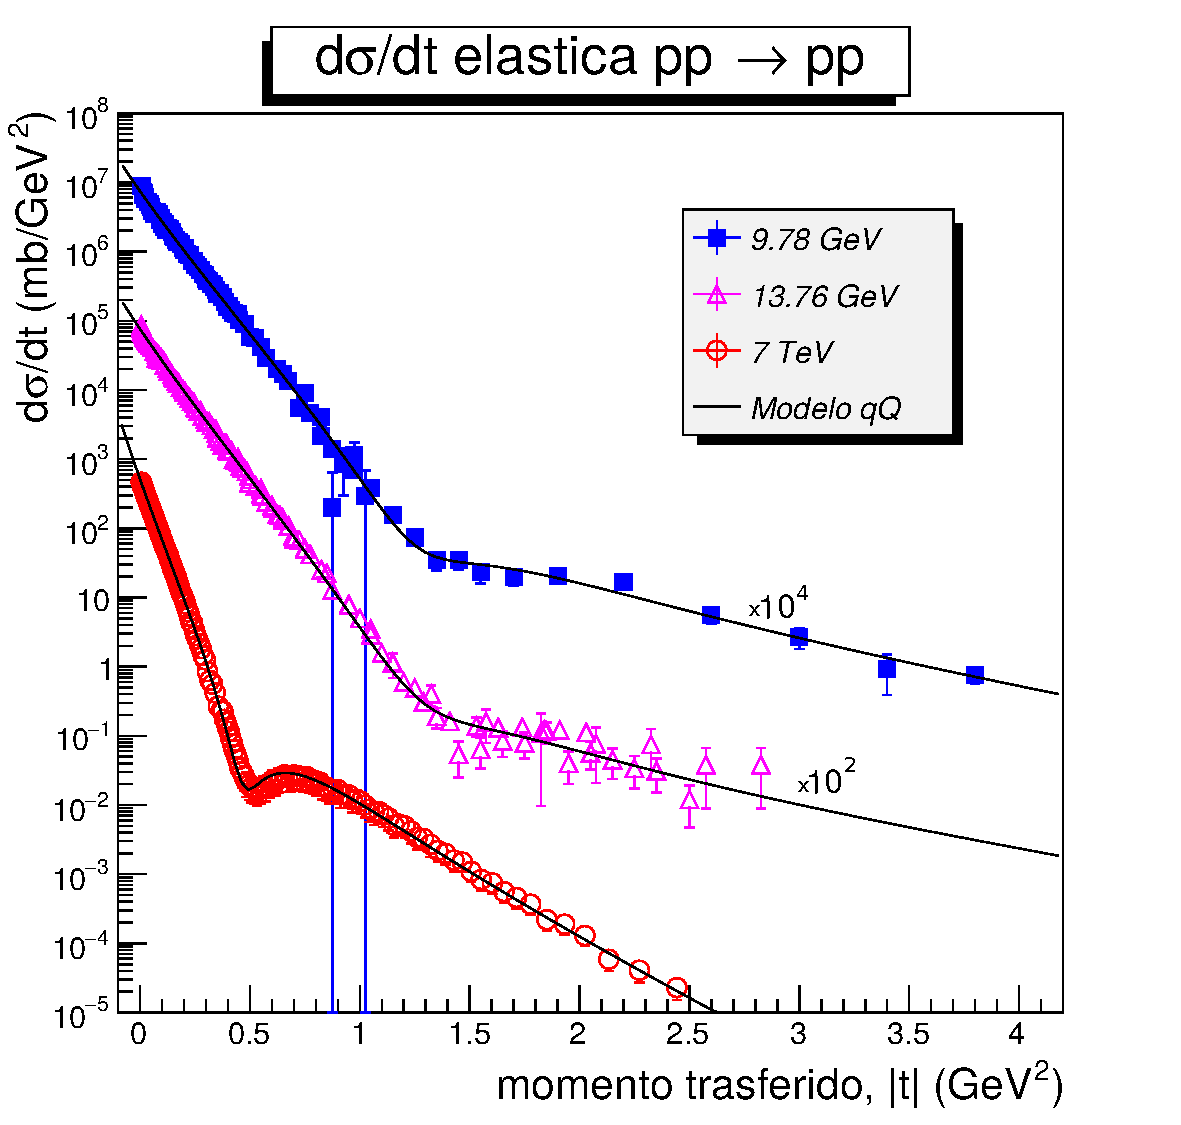
\includegraphics[width=8.8cm]{graficas/unnamedp.pdf}
\caption{\mismall Ajustes para datos de $d\sigma_{el}/dt$ en colisiones prot\'on-prot\'on en un rango de energías de colisión entre: 9.78 GeV, 13.76 GeV y 7 TeV. La escala vertical ha sido normalizada de manera diferente para diferenciar los datos de cada energía.}
\label{lafig_1}
\end{figure}
La figura \ref{lafig_radioprotonNg} muestra los valores obtenidos  para el radio del protón, $r$, en función de $\sqrt{s}$, donde se demuestra el incremento del radio del protón a medida que la energía de colisión aumenta.%\vskip -0.0cm
\begin{figure}[H]\centering
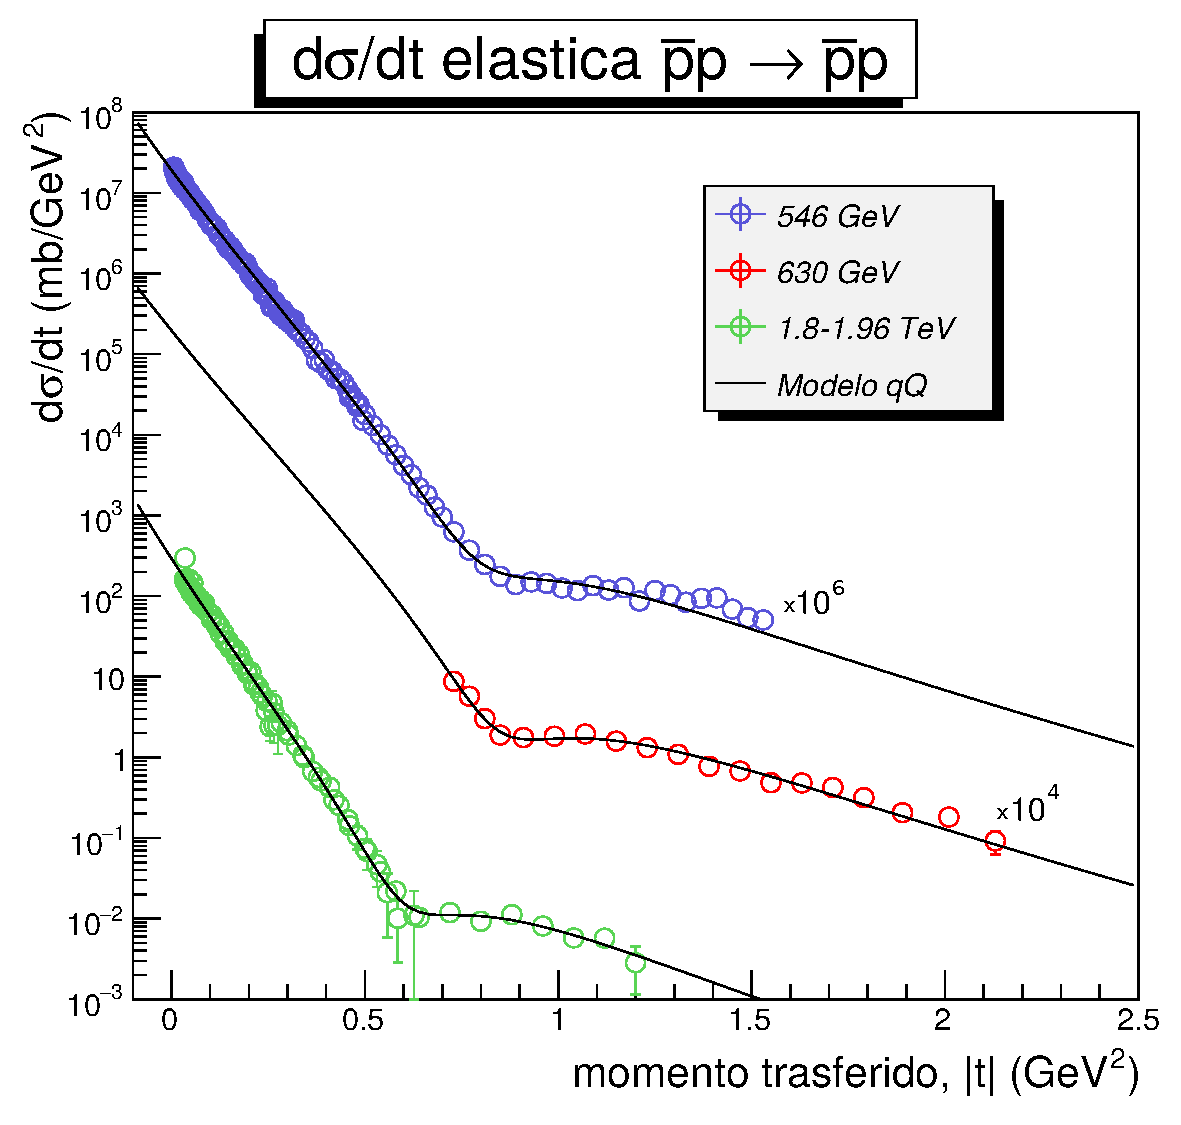
\includegraphics[width=8.5cm]{graficas/unnamedpbarp.pdf}
\caption{\mismall Ajustes para datos de $d\sigma_{el}/dt$ en colisiones prot\'on-antiprot\'on en un rango de energías de colisión entre: 546 GeV-1960 GeV. La escala vertical ha sido normalizada de manera diferente para diferenciar los datos de cada energía.}
\label{lafig_2}
\end{figure}\vskip -0.5cm
\begin{figure}[H]\centering
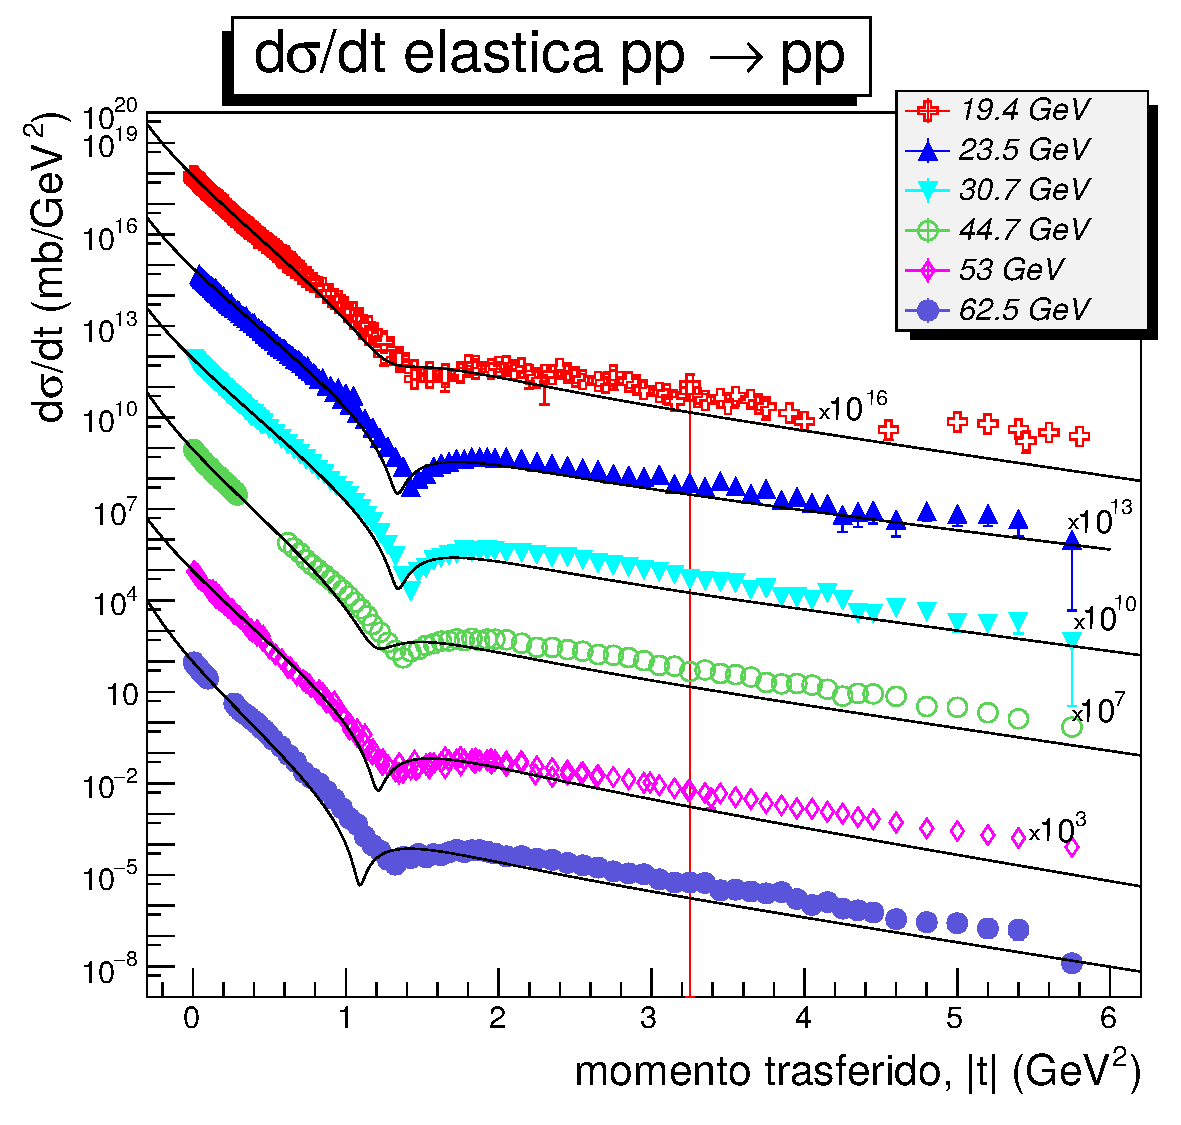
\includegraphics[width=8.5cm]{graficas/multifitgraf.pdf}
\caption{\mismall Ajustes para datos de $d\sigma_{el}/dt$ en colisiones prot\'on-prot\'on en un rango de energías de colisión entre: 19.4 GeV-62.5 GeV. La escala vertical ha sido normalizada de manera diferente para diferenciar los datos de cada energía.}
\label{lafig_3}
\end{figure}%\vskip -0.5cm
Por otra parte, cuando se ajustan datos de $d\sigma/dt$ en un intervalo mas peque\~no para $|t|$, se puede ver que el modelo brinda una mejor descripción  a los datos experimentales correspondientes a energías entre: 19.4 GeV y 62.5 GeV, las figuras \ref{lafig_6} y \ref{lafig_7} lo demuestran (observe que $\chi^2/$ndf es mas próximo a 1). Los resultados que se obtienen en los ajustes para las otras energías son similares y se encuentran listados en la tabla \ref{table2}. Los datos de color azul se encuentran en un intervalo para $|t|$ entre 0.005 GeV$^2$ y 1.0 GeV$^2$ y los datos de color negro en un intervalo para $|t|$ entre 1.0 GeV$^2<|t|<   \textup{6.0 GeV}^2$, este fue el intervalo para el cual el modelo puede hacer un mejor ajuste.
\begin{figure}[H]\centering
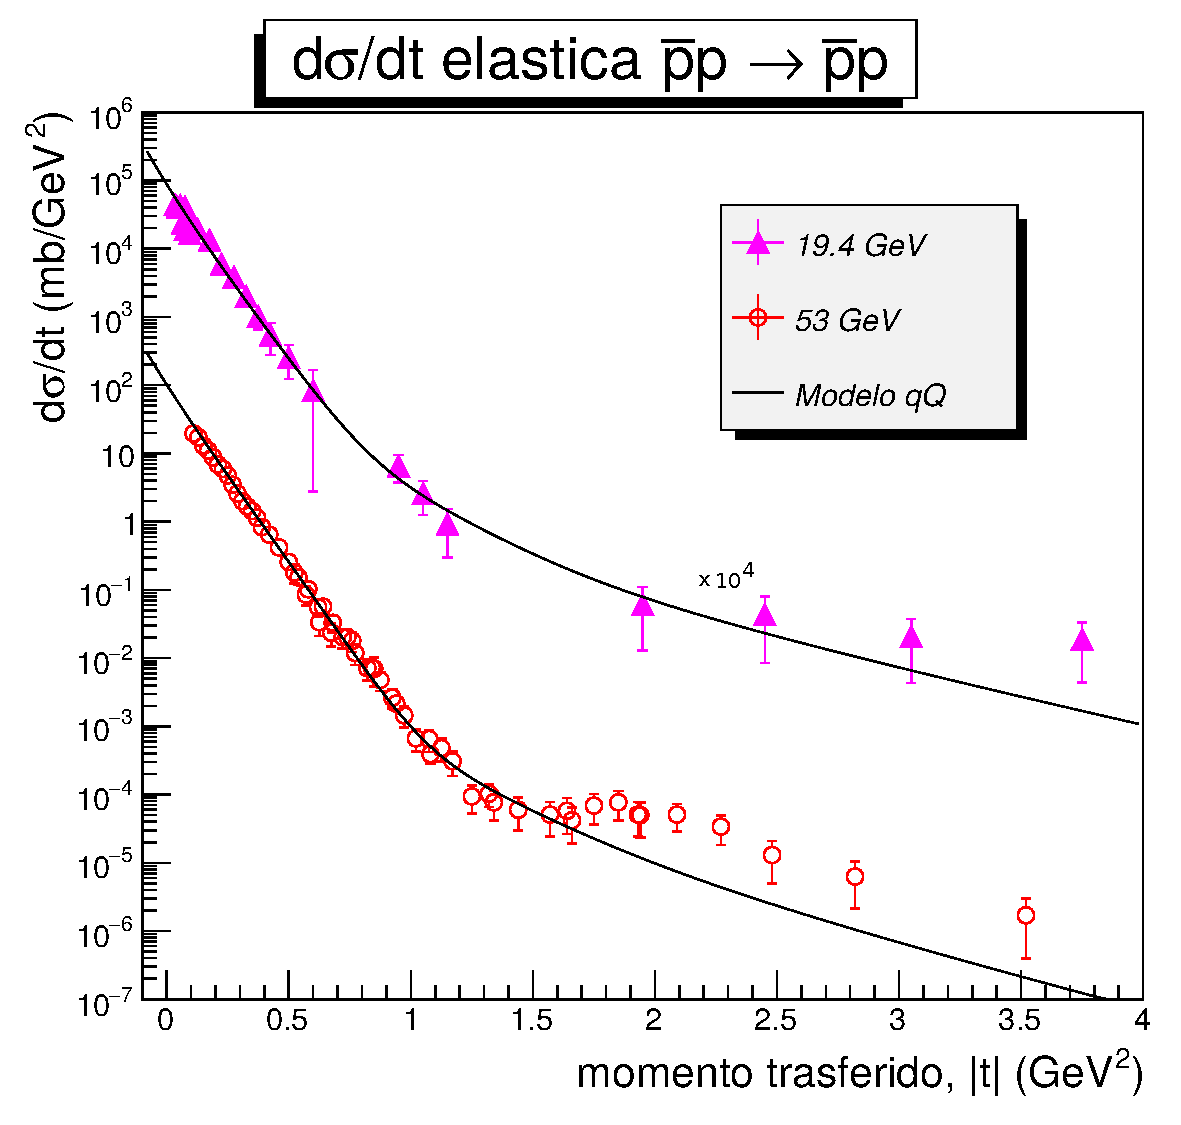
\includegraphics[width=8.5cm]{graficas/unnamed1pbar.pdf}
\caption{\mismall Ajustes para datos de $d\sigma_{el}/dt$ en colisiones prot\'on-antiprot\'on en un rango de energías de colisión entre: 19.4 GeV-53 GeV. La escala vertical ha sido normalizada de manera diferente para diferenciar los datos de cada energía.}
\label{lafig_4}
\end{figure}%\vskip -0.4cm
\begin{table}[H]
\begin{center}
\caption{\mismall Parámetros obtenidos en los ajustes en colisiones prot\'on-prot\'on y antiprot\'on-prot\'on. $r$ se mide en GeV$^{-1}$ y $\sqrt{s}$ en GeV. }
\label{table1}\mmismall
\begin{tabular}{c c c c c c c}\\
\noalign{\hrule height 0.5pt}
\toprule % <-- Toprule here
\multicolumn{4}{c}{Colisiones prot\'on-prot\'on}\\
\hline
\mmismall$\sqrt{s}$& $r$ & $\alpha_{p}$&$B_{13}$& $\frac{\chi^2}{\textup{ndf}}$\\ 
\hline 
%#######################################################################################
9.78	 &	 7.49$\pm$ 0.17	 & 	  6.4$\pm$  0.4	 &	(1.55$\pm$0.07)$\times 10^{-2}$	  & 	1.8\\ 
13.76	 &	 7.66$\pm$ 0.16		 & 	   7.0$\pm$  0.5  &	(1.07$\pm$0.05)$\times 10^{-2}$	  & 	2.0\\ 
19.4	 &	 7.84$\pm$ 0.09	 & 	  3.8$\pm$  0.4	 &	(8.2$\pm$0.3)$\times 10^{-3}$	      & 	3.9\\ 
23.5	 &	 7.72$\pm$ 0.07	 & 	  1.0$\pm$  0.2	 &	(8.6$\pm$0.1)$\times 10^{-3}$	   & 	13.8\\ 
30.7	 &	 7.75$\pm$ 0.07	 & 	  1.0$\pm$  0.1	 &	(7.4$\pm$0.8)$\times 10^{-3}	$& 	18.2\\ 
44.7	 &	 8.03$\pm$ 0.09	 & 	  4.2$\pm$  0.3 &	(8.6$\pm$0.2)$\times 10^{-3}	$& 	12.5\\ 
53.0	 &	 7.67$\pm$ 0.09	 & 	  1.0$\pm$  0.1	 &	(1.120$\pm$0.008)$\times 10^{-2}$	& 	9.6\\ 
62.5	 &	 8.15$\pm$ 0.11	 & 	  1.0$\pm$  0.2	 &	(1.24$\pm$0.02)$\times 10^{-2}$	& 	11.3\\ 
7000	 &	 8.70$\pm$ 0.18	 & 	  7.1$\pm$  0.6	 &	(4.59$\pm$0.07)$\times 10^{-2}$	& 	0.8\\ 
\hline
\multicolumn{4}{c}{Colisiones antiprot\'on-prot\'on}\\
\hline
19.4	 &	 8.16$\pm$ 1.01	 & 	  9.0$\pm$  1.1	 &	(2.2$\pm$0.4)$\times 10^{-2}$	& 	2.0\\ 
53  	 &	 8.16$\pm$ 0.24	 & 	  9.0$\pm$  0.3	 &	(9.0$\pm$0.7)$\times 10^{-3}	$	& 	1.2\\ 
546	     &	 7.97$\pm$ 0.17	 & 	  7.6$\pm$  0.3	 &	(2.23$\pm$0.05)$\times 10^{-2}$	& 	1.6\\ 
630	     &	 7.56$\pm$ 0.55	 & 	  6.1$\pm$  0.4	 &	(2.27$\pm$0.07)$\times 10^{-2}$	& 	0.6\\ 
1800	 &	 8.03$\pm$ 0.35	 & 	  8.0$\pm$  1.0	 &	(3.9$\pm$0.1)$\times 10^{-2}$	& 	1.6\\ 
%########################################################################################
%\hline
\bottomrule % <-- Bottomrule here
\noalign{\hrule height 0.5pt}
 \end{tabular}
\end{center}
\end{table}\vskip -0.5cm
\begin{figure}[H]\centering
\includegraphics[width=8cm]{graficas/radioproton.pdf}
\caption{Variación de $r$ como función de la energía de colisión $\sqrt{s}$.}
\label{lafig_radioprotonNg}
\end{figure}
En estos fits puede verse que los datos no son bien descritos por la amplitud de dispersión propuesta a valores de $|t|<$1.0 GeV$^2$, en las figuras \ref{lafig_6} o \ref{lafig_7} podemos ver que la curva del modelo presenta una peque\~na concavidad con pendiente negativa antes de llegar al m\'inimo de difracción, generándose una sobre-estimación en este intervalo.
%\begin{figure}[H]\centering
%\includegraphics[width=8cm]{/home/alejandro/Escritorio/articulodoc/graficas/radioproton.pdf}
%\caption{La dependencia de $\ln(r)$, ($r$ en GeV$^{-1}$) de $\ln\left(\sqrt{s/s_{0}}\right)$.}
%\label{lafig_radioproton}
%\end{figure}
%La parametrizaci\'on para la curva de la figura \ref{lafig_radioproton} es:
%\begin{equation}
%\ln(r)=\textup{2.03}\pm \textup{0.01}+(\textup{0.017}\pm \textup{0.005})\ln\left(\sqrt{\frac{s}{s_0}}\right)
%\end{equation}
\begin{table}[H]
\begin{center}
\caption{\mismall Parámetros obtenidos en los ajustes en colisiones prot\'on-prot\'on y antiprot\'on-prot\'on. $r$ se mide en GeV$^{-1}$ y $\sqrt{s}$ en GeV. }
\label{table2}\mmismall
\begin{tabular}{c c c c c}\\
\noalign{\hrule height 0.5pt}
\toprule % <-- Toprule here
\multicolumn{4}{c}{Colisiones prot\'on-prot\'on}\\
\hline
%\begin{sideways}columna 1\end{sideways}&\begin{sideways}columna 2 \end{sideways} 
\mismall$\sqrt{s}$&$r$&$\alpha_{p}$&$B_{13}$&$\frac{\chi^2}{ndf}$\\ 
\hline
19.4&7.42$\pm$0.02&2.1$\pm$ 0.2	&(7.5$\pm$0.1)$\times 10^{-3}$&2.3\\ 
23.5&7.355$\pm$0.009&1.01$\pm$ 0.09	&(8.35$\pm$0.07)$\times 10^{-3}$&3.8\\ 
30.7&7.343$\pm$0.008&0.65$\pm$ 0.02	&(7.96$\pm$0.06)$\times 10^{-3}$&4.7\\ 
44.7&7.407$\pm$0.008&1.2$\pm$ 0.1	&(9.22$\pm$0.07)$\times 10^{-3}$&8.6\\ 
53.0&7.303$\pm$0.008&1.81$\pm$ 0.03	&(9.60$\pm$0.05)$\times 10^{-3}$&8.5\\ 
62.5&7.44$\pm$0.01&1.80$\pm$ 0.03	&(9.6$\pm$0.1)$\times 10^{-3}$&5.8\\
\hline
\multicolumn{4}{c}{Colisiones antiprot\'on-prot\'on}\\
\hline
19.4	 &	7.3$\pm$0.1	 & 	 1.5$\pm$6.1	 &	(9.5$\pm$2.0)$\times 10^{-3}$&0.5\\ 
53.0	 &	7.8$\pm$0.1	 & 	 4.9$\pm$ 1.0	 &	(8.6$\pm$0.6)$\times 10^{-3}$&0.7\\ 
\bottomrule % <-- Bottomrule here
\noalign{\hrule height 0.5pt}
 \end{tabular}
\end{center}
\end{table}\vskip -0.4cm
\begin{figure}[H]\centering
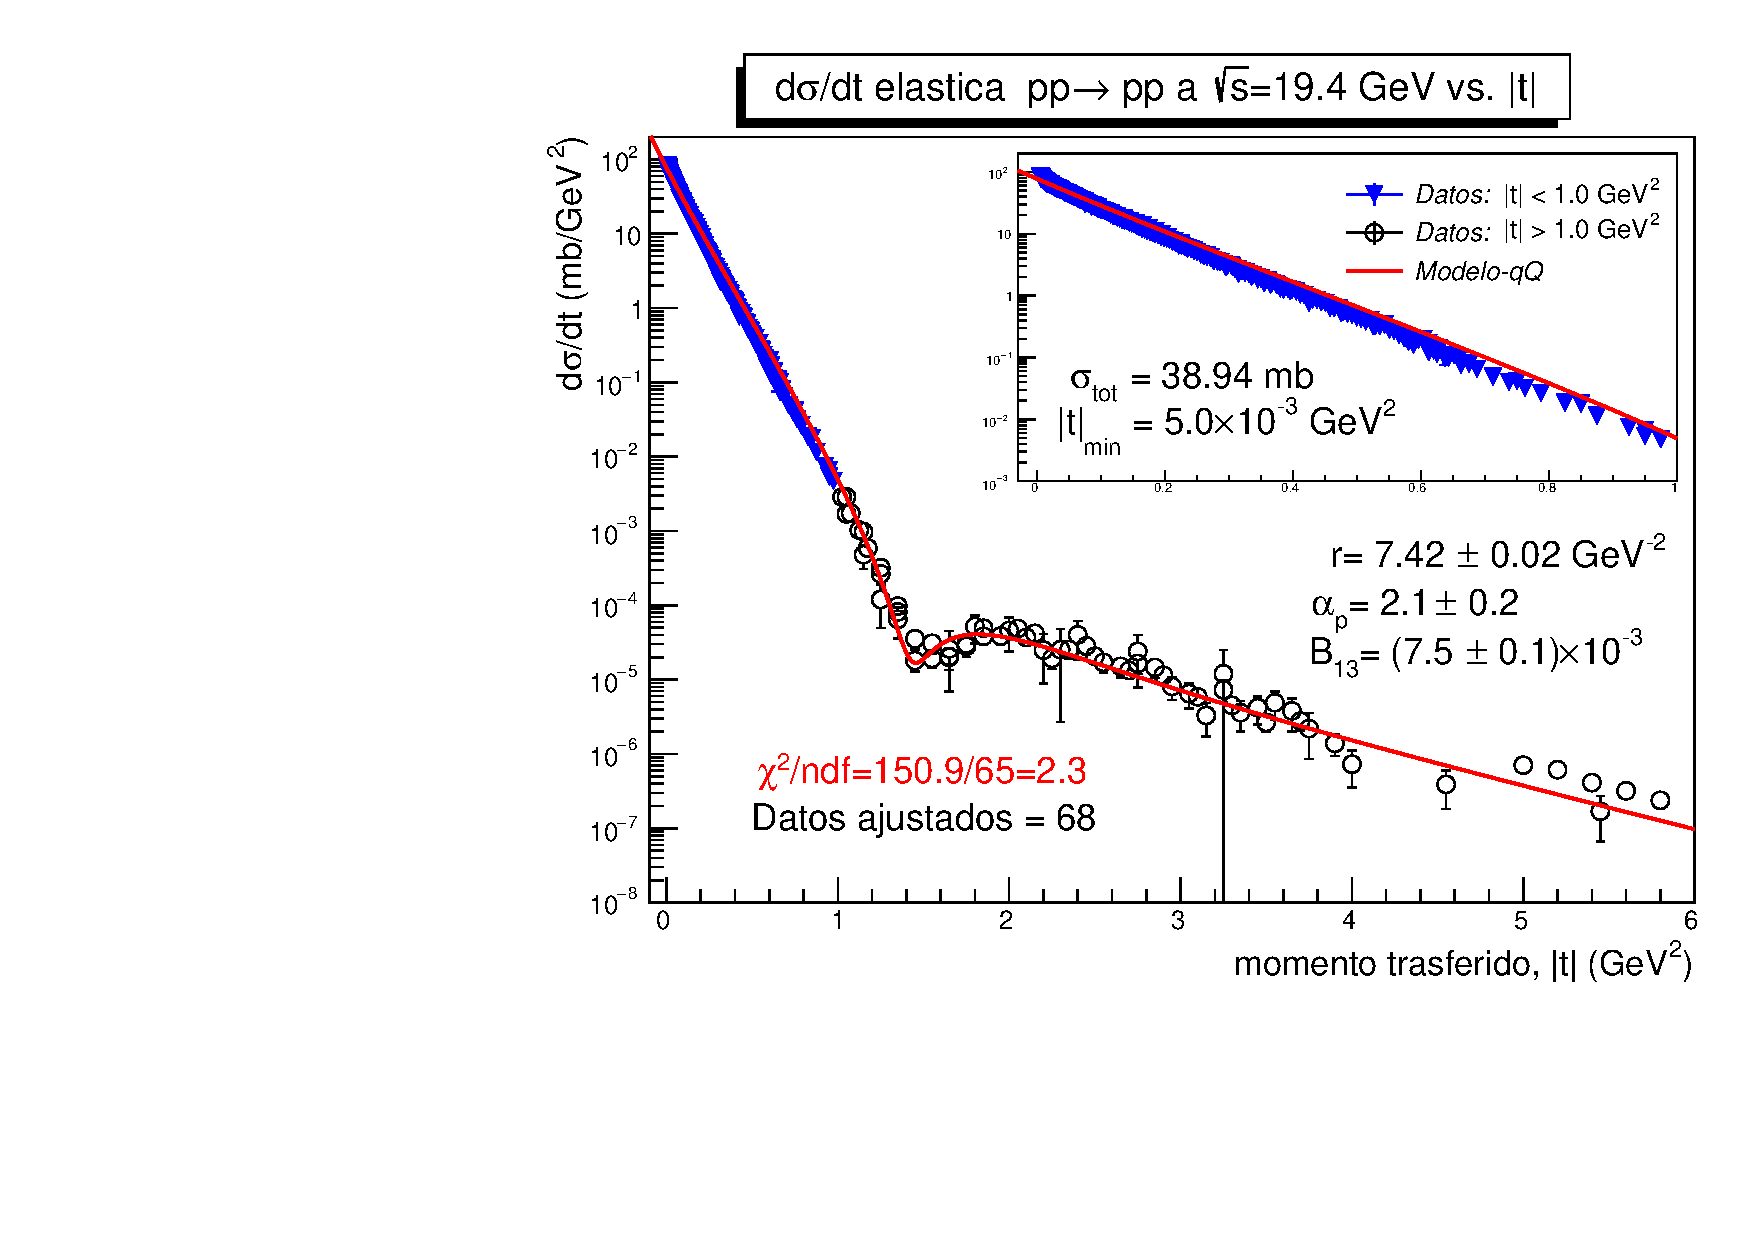
\includegraphics[width=7.9cm]{graficas/ajuste19pp.pdf}
\caption{\mismall Ajuste a los datos de sección eficaz diferencial elástica en colisiones prot\'on-prot\'on a $\sqrt{s}=19\textup{.}4$ GeV. La curva es el modelo $qQ_{-}$ con pomer\'on elástico para el intervalo de ajuste 1.0 GeV$^2<|t|<\textup{6.0 GeV}^2$.}
\label{lafig_6}
\end{figure}\vskip -0.5cm
\begin{figure}[H]\centering
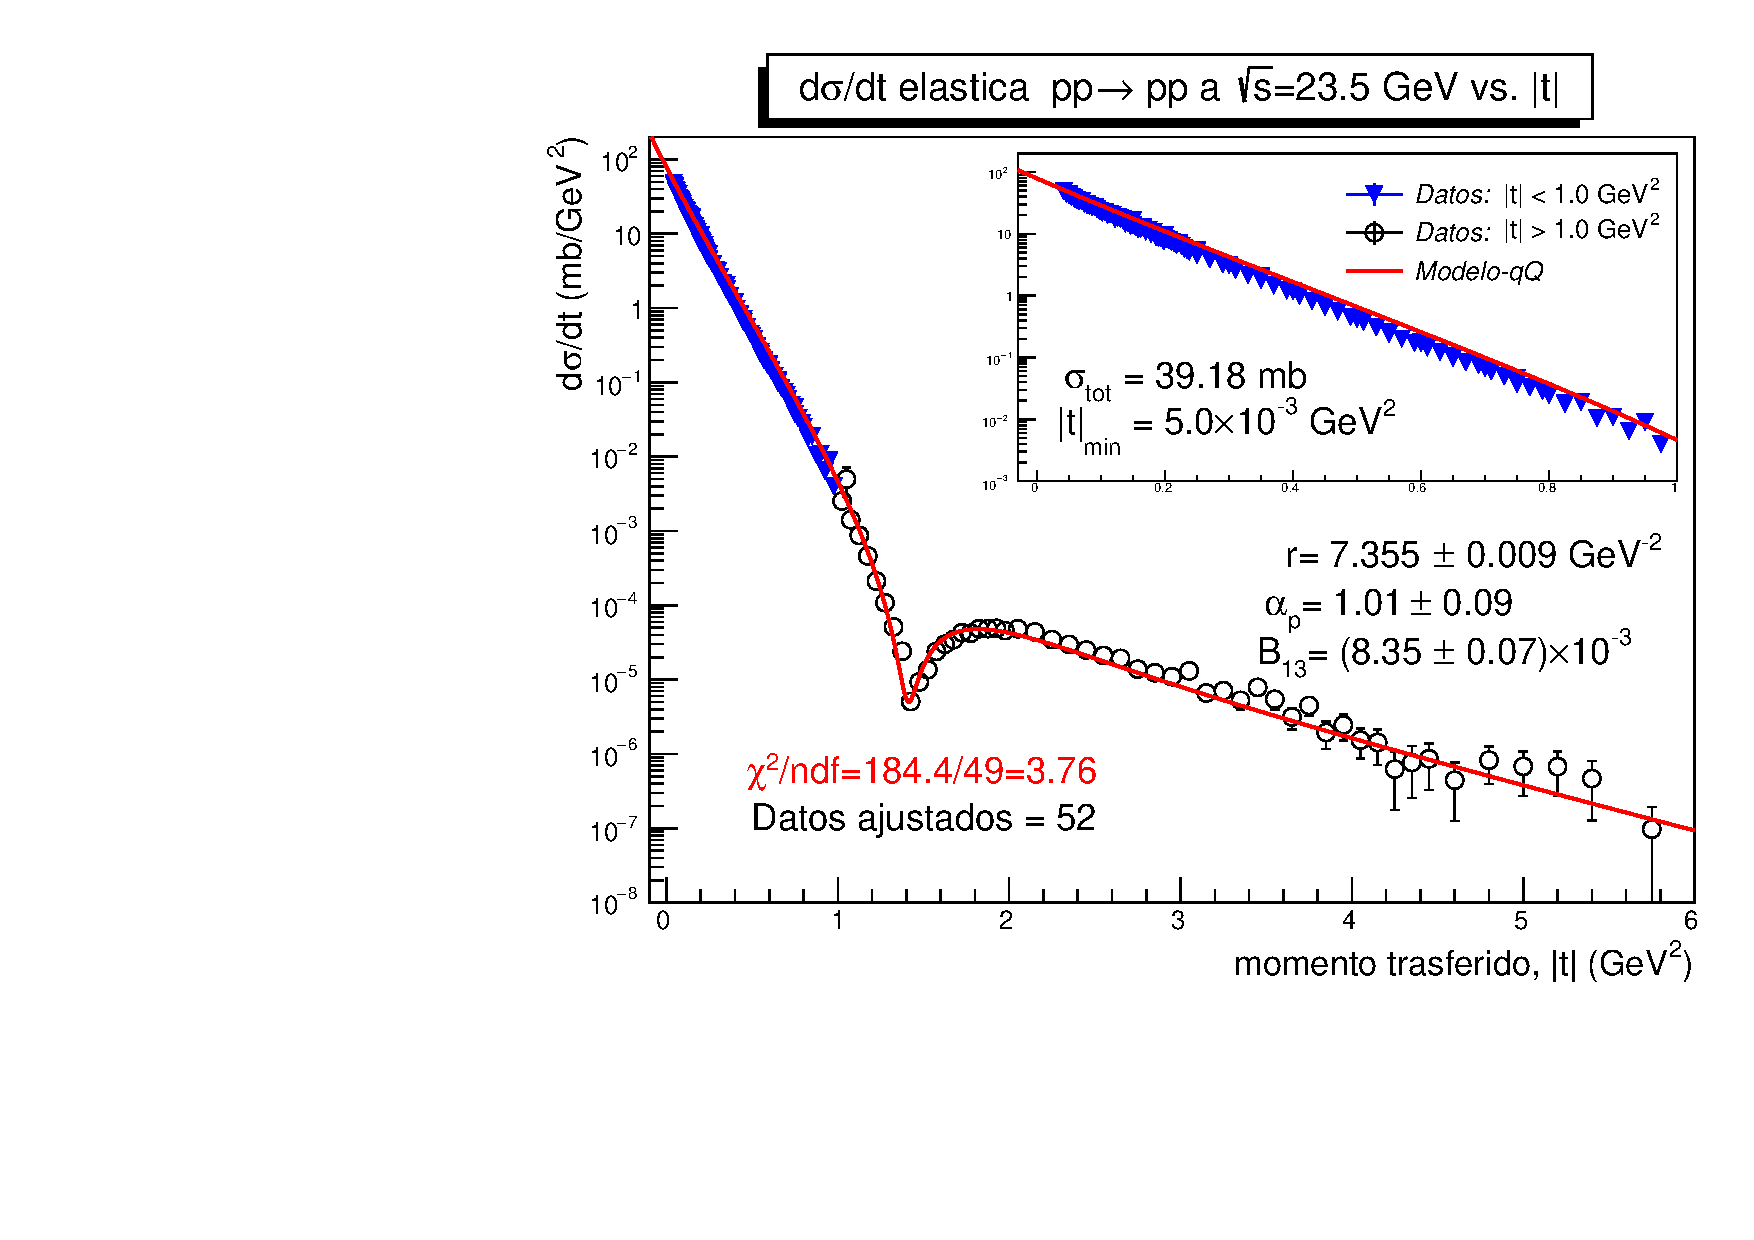
\includegraphics[width=7.9cm]{graficas/ajuste23pp.pdf}
\caption{\mismall Ajuste a los datos de sección eficaz diferencial elástica en colisiones prot\'on-prot\'on a $\sqrt{s}=23\textup{.}5$ GeV. La curva es el modelo $qQ_{-}$ con pomer\'on elástico para el intervalo de ajuste 1.0 GeV$^2<|t|<\textup{6.0 GeV}^2$.}
\label{lafig_7}
\end{figure}%\vskip -0.3cm
\section{Modelo qQ$_{-}$ y $\mathcal{N_{G}}(s)$}
El problema de la amplitud de dispersión propuesta por Grichine es que la normalización global est\'a fija y el ajuste falla en la descripción correcta del mínimo de difracción, en este trabajo se propone dejar como parámetro libre est\'a normalización global, es decir, la ecuación \ref{ecu2f} ahora ser\'ia de la forma:
\begin{equation}
F(s,t)=\mathcal{N_G}(s)[F_1(s,t)-F_2(s,t)-F_3(s,t)]
\end{equation}
y a partir del teorema óptico podemos ver que:
\begin{equation}
\sigma_{tot}=\frac{4\pi}{p}\textup{Im}\{\mathcal{N_G}(s)[F_1(s,0)-F_2(s,0)-F_3(s,0)]\}
\end{equation}
c\'omo $\mathcal{N_G}(s)$ es un n\'umero real positivo, entonces: 
\begin{equation}
\frac{4\pi}{p}\textup{Im}\{[F_1(s,0)-F_2(s,0)-F_3(s,0)]\}-\frac{\sigma_{tot}}{\mathcal{N_G}(s)}=0
\end{equation}
en consecuencia, el coeficiente $a_0$ en las ecuaciones (\ref{misecu5}) es de la forma:
\begin{equation}
a_0=\frac{1}{\mathcal{N_G}(s)}-B_{13}
\end{equation}
\'Este nuevo parámetro permite que el modelo pueda ajustar los datos en un amplio rango de energías, desde 9.7 GeV a 7 TeV en colisiones pp y desde 19.4 GeV a 1960 GeV en colisiones $\bar{\textup{p}}$p, las figuras \ref{lafig_14} y \ref{lafig_15} muestran los ajustes realizados con estos 4 parámetros: radio del prot\'on, elasticidad del pomer\'on, coeficiente de pendiente nuclear, y normalización global. En la tabla \ref{table3} se muestran los parámetros obtenidos en los ajustes mostrados en las figuras \ref{lafig_14} y \ref{lafig_15} con sus respectivos $\chi^2/$ndf. Aquí podemos ver que los ajustes mejoran considerablemente.
Finalmente, en la  figura \ref{lafig_sigma}  mostramos la variación de $B_{13}=\sigma_{13}/\sigma_{tot}$  en funci\'on de $\sqrt{s}$, respectivamente. 
\begin{figure}[H]\centering
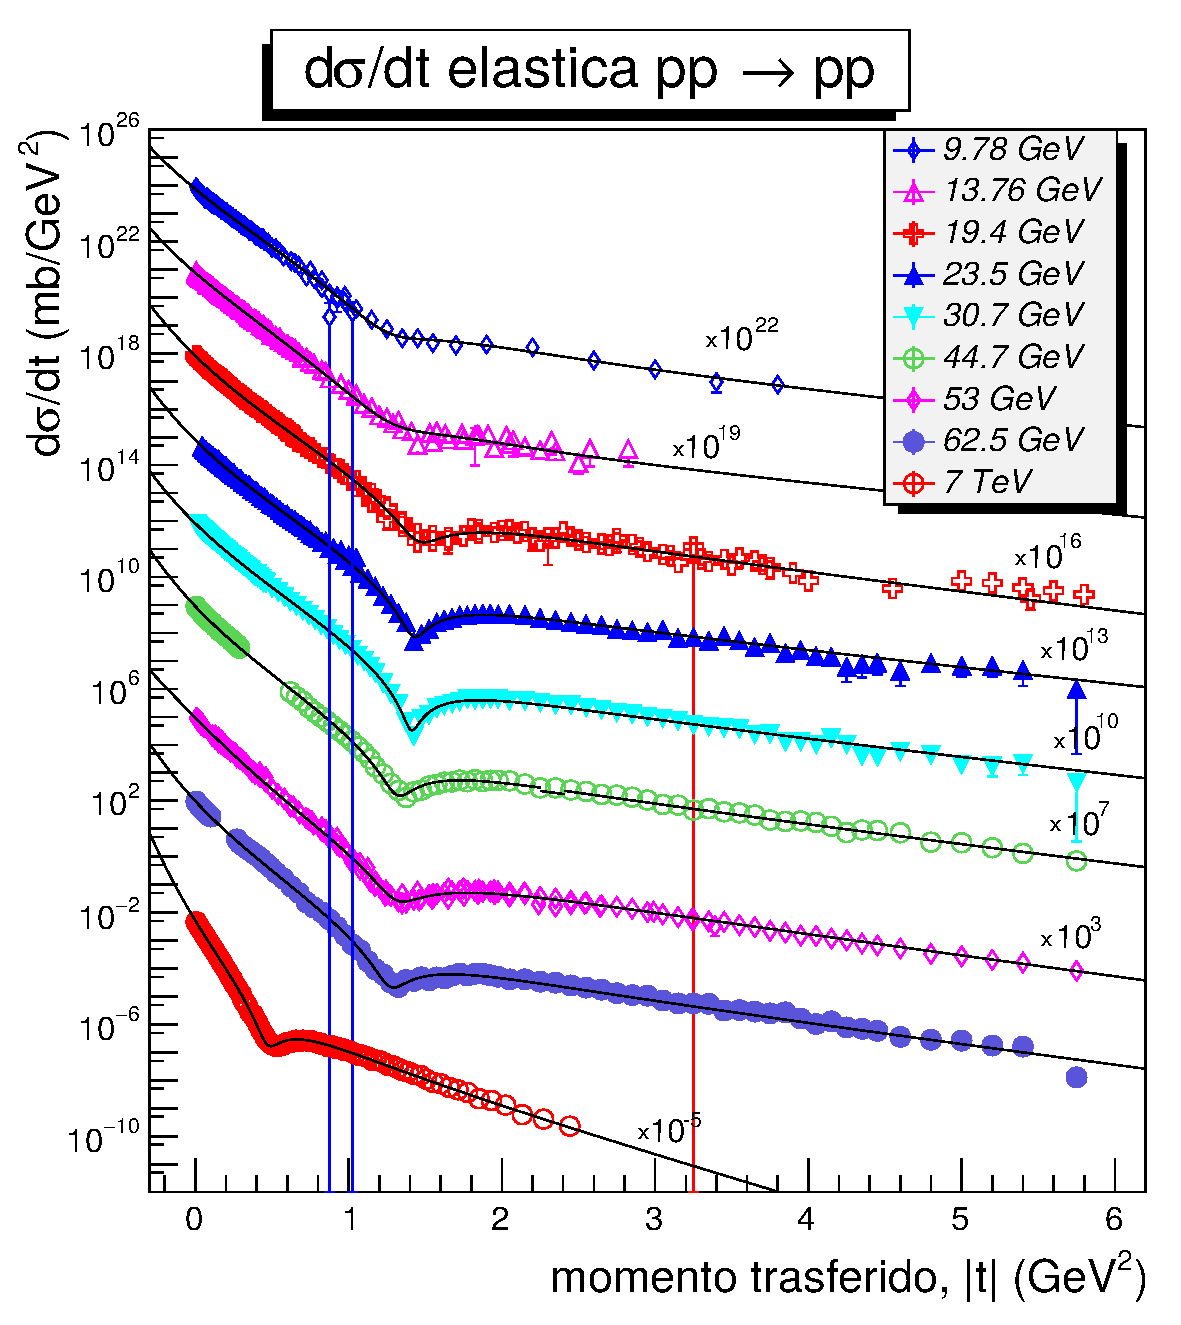
\includegraphics[width=8cm]{graficas/multifit.pdf}
\caption{\mismall Ajustes para datos de $d\sigma_{el}/dt$ en colisiones prot\'on-prot\'on en un rango de energías de colisión entre: 9.78 GeV y 7 TeV. La escala vertical ha sido normalizada de manera diferente para diferenciar los datos de cada energía.}
\label{lafig_14}
\end{figure}%\vskip -0.5cm
\begin{figure}[H]\centering
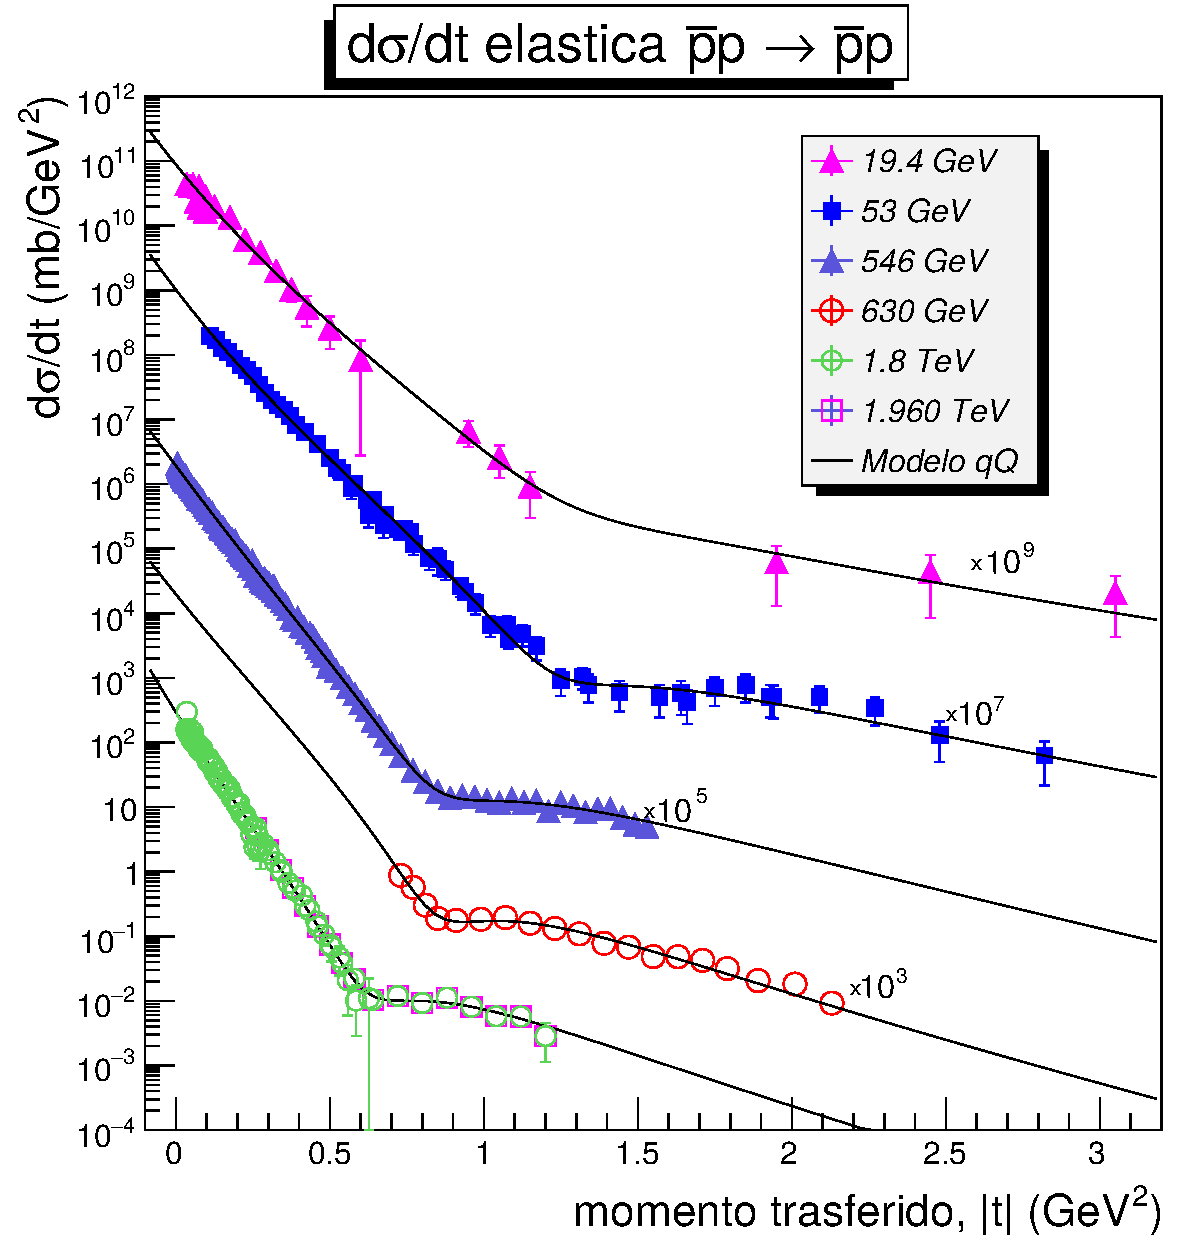
\includegraphics[width=7.9cm]{graficas/multifitl.pdf}
\caption{\mismall Ajustes para datos de $d\sigma_{el}/dt$ en colisiones prot\'on-prot\'on en un rango de energías de colisión entre: 19.4 GeV y 1960 GeV. La escala vertical ha sido normalizada de manera diferente para diferenciar los datos de cada energía.}
\label{lafig_15}
\end{figure}\vskip -0.5cm
%\begin{tabular}{p{3cm}p{10cm}p{3cm}}
%\hline 
%\begin{minipage}[r]{5cm}
%\end{minipage}
 %& \begin{minipage}[r]{10cm}
 \begin{table}[H]
\begin{center}
\caption{\mismall Parámetros obtenidos en los ajustes en colisiones prot\'on-prot\'on y antiprot\'on-prot\'on. $r$ se mide en GeV$^{-1}$ y $\sqrt{s}$ en GeV.}
\label{table3}\mmismall
\begin{tabular}{c c c c c c c}\\
\noalign{\hrule height 0.5pt}
\toprule % <-- Toprule here
\multicolumn{5}{c}{\bf Colisiones prot\'on-prot\'on}\\
\hline
\mmismall$\sqrt{s}$& $r$ & $\alpha_{p}$&$B_{13}$&$\mathcal{N_{G}}(s)$& $\frac{\chi^2}{\textup{ndf}}$\\ 
&&&$\times 10^{-2}$ &&\\
\hline 
%#######################################################################################
9.8	 &	 7.43$\pm$ 0.02	 & 	  6.1$\pm$  0.5	     &  1.25$\pm$0.06	&1.2$\pm$	0.1& 	1.9\\ 
13.8	 &	 7.47$\pm$ 0.04	 & 	  5.9$\pm$  0.6	 &	1.10$\pm$0.05	&1.9$\pm$	0.2&	1.7\\ 
19.4	 &	 7.35$\pm$ 0.02	 & 	  3.0$\pm$  0.2	 &	1.05$\pm$0.02 &3.9$\pm$	0.2& 	1.8\\ 
23.5	 &	 7.14$\pm$ 0.02	 & 	  1.4$\pm$  0.1	 &	1.38$\pm$0.02	&4.9$\pm$	0.1& 	1.0\\ 
30.7	 &	 7.20$\pm$ 0.01	 & 	  1.0$\pm$  0.1	 &	1.25$\pm$0.01	&4.3$\pm$	0.1& 	1.5\\ 
44.7	 &	 7.20$\pm$ 0.02	 & 	  2.0$\pm$  0.1	 &	1.55$\pm$0.02 &4.9$\pm$	0.1& 	4.9\\ 
53	 &	 7.17$\pm$ 0.02	 & 	  1.9$\pm$  0.1	 &	1.65$\pm$0.02     & 4.6$\pm$	0.1&	3.5\\ 
62.5	 &	 7.22$\pm$ 0.02	 & 	  2.2$\pm$  0.2	 &	1.60$\pm$0.02	&4.7$\pm$	0.1& 	2.4\\ 
7000	 &	 8.52$\pm$ 0.02	 & 	  7.9$\pm$  0.5	 &	4.67$\pm$0.08	&1.2$\pm$	0.1& 	0.8\\ 

\hline
\multicolumn{5}{c}{\bf Colisiones antiprot\'on-prot\'on}\\
\hline
19.4	 &	 6.78$\pm$ 0.33	 & 	  5.4$\pm$  6.2	 &	2.0$\pm$0.7	&9.2$\pm$	3.6& 	1.7\\ 
53	 &	 7.50$\pm$ 0.14	 & 	  6.3$\pm$  1.0	 &	1.4$\pm$0.2	&9.8$\pm$	1.1& 	0.5\\ 
546	 &	 7.78$\pm$ 0.05	 & 	  7.1$\pm$  0.3	 &	2.5$\pm$0.1	&1.4$\pm$	0.1& 	1.5\\ 
630	 &	 7.52$\pm$ 0.13	 & 	  6.5$\pm$  1.0	 &	2.4$\pm$0.7	&1.3$\pm$	1.2& 	0.5\\ 
1800	 &	 7.81$\pm$ 0.04	 & 	  8.3$\pm$  0.4	 &	4.5$\pm$0.1	&1.2$\pm$	0.0& 	1.9\\ 

%########################################################################################
%\hline
\bottomrule % <-- Bottomrule here
\noalign{\hrule height 0.5pt}
 \end{tabular}
\end{center}
\end{table}
%\end{minipage} & \begin{minipage}[r]{5cm}
%\end{minipage} \\ 
%\hline 
%\end{tabular} 
\vskip -0.5cm
\begin{figure}[H]\centering
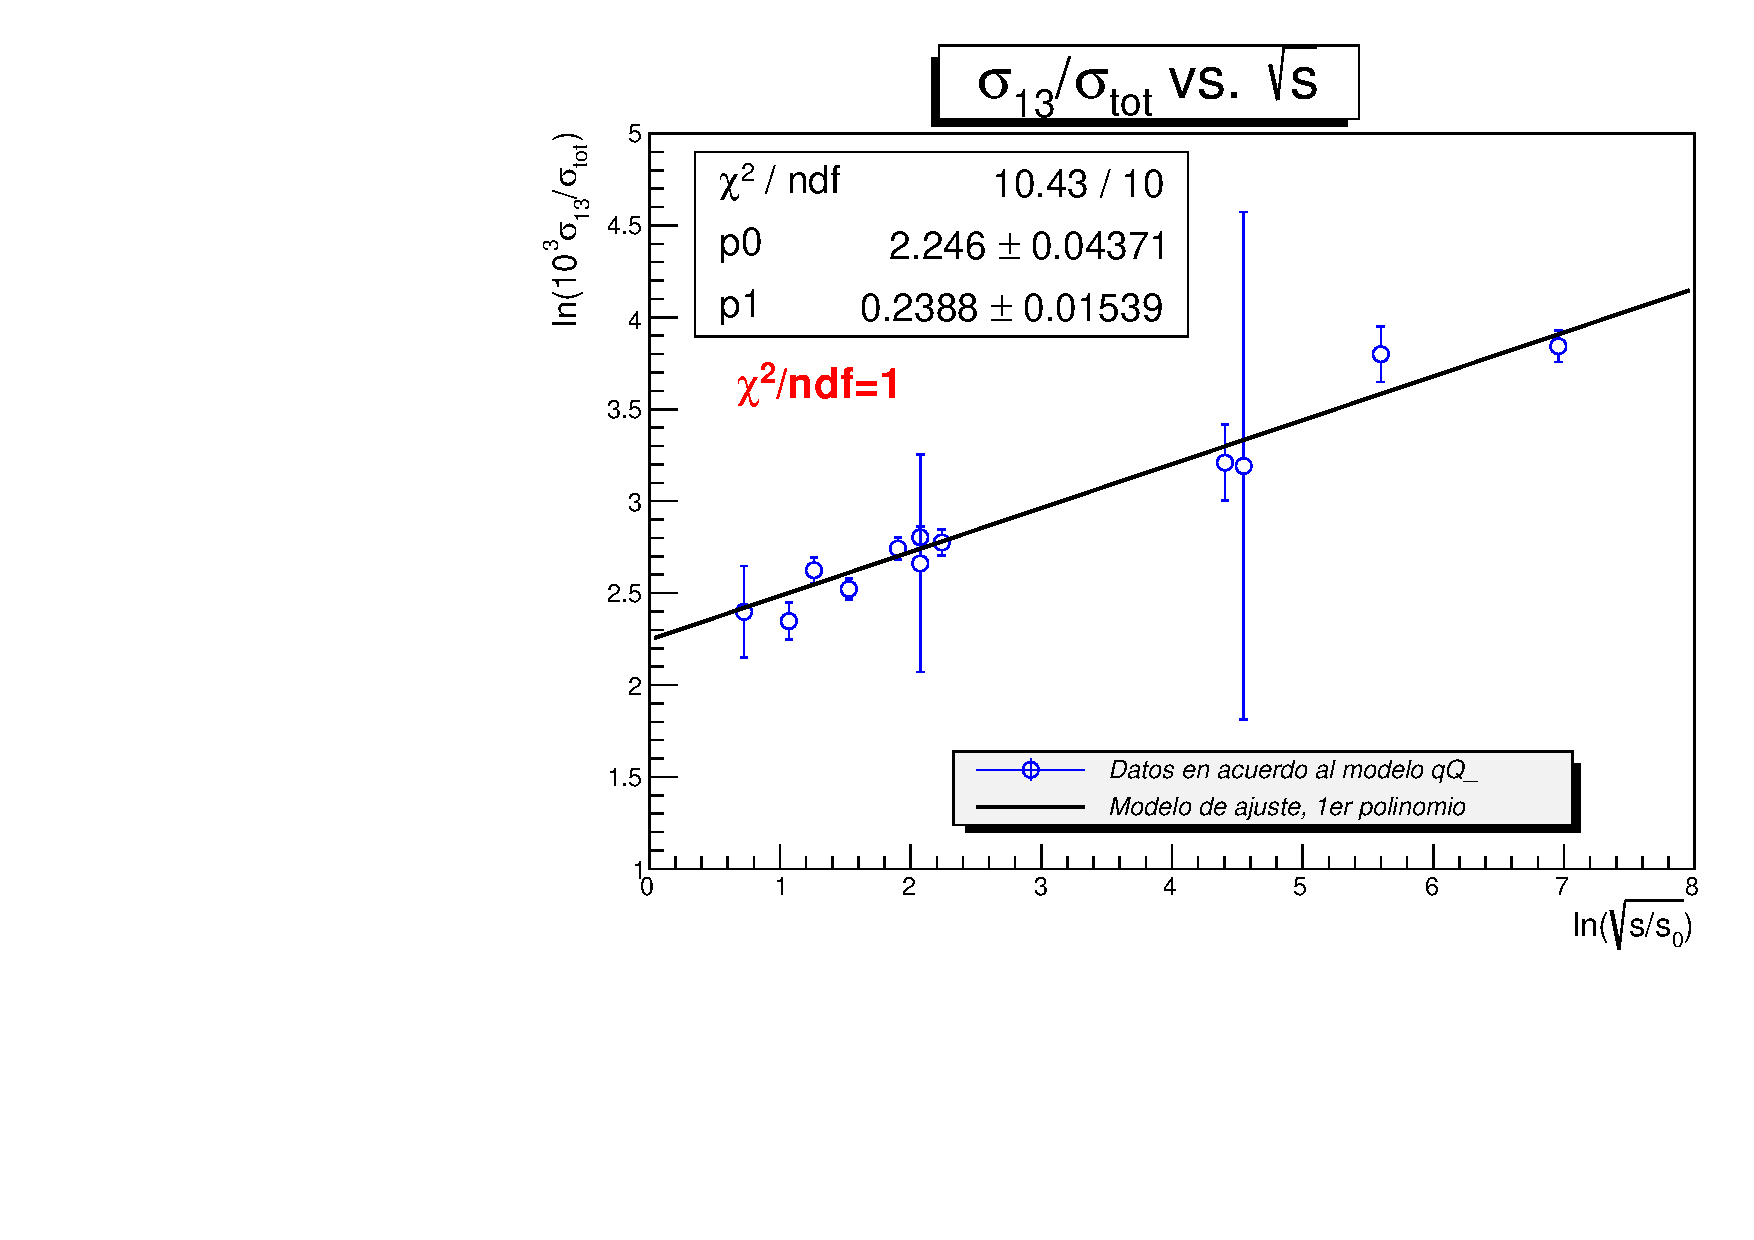
\includegraphics[width=8cm]{graficas/grafsigma.pdf}
\caption{Dependencia de $\sigma_{13}/\sigma_{tot}$ vs. $\sqrt{s}$.}
\label{lafig_sigma}
\end{figure} 
\section{Conclusiones}
En el presente trabajo se hizo un corto estudio a un modelo de dispersión
elástica de nucleones, particularizado a los protones. A lo largo de su desarrollo probamos que el modelo que propone Grichine para la descripción de datos de sección eficaz diferencial elástica, tiene dificultades  en determinar la posición del mínimo de difracción a ciertas energías intermedias en colisiones protón-protón y antiprot\'on-prot\'on.\\

\ \ Nuestro estudio muestra que para que  el modelo ($qQ$) con pomerón elástico describa apropiadamente todos los datos accesibles de sección eficaz diferencial para dispersión elástica prot\'on-prot\'on y antiprot\'on-prot\'on, se necesita una modificación a la amplitud de dispersión propuesta por Grichine. La amplitud de dispersión debe ser modificada en términos de una normalización que depende de la energía. Cuando en el ajuste incluimos un parámetro adicional correspondiente a est\'a normalización, encontramos una buena descripción de los datos.
\section*{Bibliograf\'ia}
\begin{thebibliography}{X}
%1
 \bibitem{modeloqQ} \textsc{V.M. Grichine, N.I. Starkov y N.P. Zotov.}
 \textit{Quark-diquark model for $p(\bar{p})-p$ elastic scattering at high
energies}. \textup{Eur. phys. J. C73 (2013)2320}.\\
 \href{http://lanl.arxiv.org/abs/1212.2111v2}{\texttt{arXiv:1212.2111}}

 \bibitem{grichine} \textsc{V.M. Grichine.}
 \textit{Nucleon elastic scattering in quark-diquark representation with
springy Pomeron}. \textup{Lebedev Physical Institute, Moscow, Russia, 2014}.\\
 \href{https://arxiv.org/abs/1404.5768v1}{arXiv:1404.5768}
 
%2 


%3

\bibitem{carlosavila} \textsc{Carlos Avila Bernal (2013).} \textit{Colisiones el\'asticas y secci\'on eficaz total hadr\'on-hadr\'on a altas energ\'ias}.
\textup{Revista de la academia colombiana de Ciencias Exactas, F\'isicas y Naturales. Diciembre 2014. }\href{https://www.raccefyn.co/index.php/raccefyn/article/viewFile/151/62}{\texttt{Rev. Acad. Colomb. }}
%\newpage
%4
\bibitem{martinov} \textsc{E. Martynov.}
 \textit{Proton (antiproton) elastic scattering at energies from FNAL to LHC
in the tripole pomeron-odderon model}. \textup{Bogolyubov Institute for Theoretical Physics, 03680 Kiev, Ukraine, 2013.} \href{https://arxiv.org/abs/1305.3093v1}{\texttt{arXiv:1305.3093}}

\bibitem{varone} \textsc{Vincenzo Barone \textup{y} Enrico Predazzi.} \textit{High-Energy Particle Diffraction}.
\textup{First published, Springer, Germany, 2002, p\'ags. 35$-$52, 83$-$104.}
%7
\bibitem{donachie} \textsc{S. Donnachie, G. Dosch, P. Landshoff y O. Nachtmann.} \textit{Pomeron Physics and QCD}.
\textup{First published, Cambridge, New York, 2002, p\'ags. 1$-$6, 47$-$60.}

%\bibitem{rusia}\textsc{N.P. Zotov, S.V. Rusakov, V.A. Tsarev, Fiz. Elem. Chastits At.
%Yadra 11, 1160 (1980)} \textit{(in Russian)}
%6


 
\end{thebibliography}

\end{document}








